\documentclass[conference]{IEEEtran}
\IEEEoverridecommandlockouts
\usepackage{cite}
\usepackage{amsmath,amssymb,amsfonts}
\usepackage{graphicx}
\usepackage{textcomp}
\usepackage{float}
\usepackage{xcolor}
\usepackage{booktabs}
\usepackage{multirow}
\usepackage{siunitx}
\usepackage{algorithm}
\usepackage{algpseudocode}
\usepackage{microtype}

\begin{document}

\title{VITAL: An End-to-End Contactless Vitals-to-Triage Pipeline with Hybrid rPPG Correction and a Measured Case for Deterministic Clinical Safety}

\author{
\begin{tabular*}{\textwidth}{@{\extracolsep{\fill}}ccc}

\textbf{Kushal Raj G S} & \textbf{Milind K} & \textbf{M Manoj} \\

\begin{tabular}{c}
Dept. of AIML\\
BMS Institute of Technology and\\
Management\\
Bengaluru, India\\
kushalrajgs@gmail.com
\end{tabular}
&
\begin{tabular}{c}
Dept. of AIML\\
BMS Institute of Technology and\\
Management\\
Bengaluru, India\\
milind\_k05@yahoo.com
\end{tabular}
&
\begin{tabular}{c}
Dept. of AIML\\
BMS Institute of Technology and\\
Management\\
Bengaluru, India\\
manoj044m@gmail.com
\end{tabular}

\\[1em]

\textbf{Pradeep K R} & \textbf{Anupama H S} & \textbf{M Krishna Prasad} \\

\begin{tabular}{c}
Dept. of AIML\\
BMS Institute of Technology and\\
Management\\
Bengaluru, India\\
pradeepkr@bmsit.in
\end{tabular}
&
\begin{tabular}{c}
Dept. of AIML\\
BMS Institute of Technology and\\
Management\\
Bengaluru, India\\
anupamahs@bmsit.in
\end{tabular}
&
\begin{tabular}{c}
Dept. of AIML\\
BMS Institute of Technology and\\
Management\\
Bengaluru, India\\
krishnamuralimk08@gmail.com
\end{tabular}

\end{tabular*}
}

\maketitle

\begin{abstract}
Contactless heart-rate sensing from a webcam is evaluated on its own, and is increasingly paired with language models trusted to reason about clinical risk straight from raw vitals. \textbf{VITAL} puts both assumptions to the test. Its rPPG pipeline -- \textbf{CHROM} corrected by a small gradient-boosted model -- reaches \textbf{6.48 BPM mean absolute error} across \textbf{71 real sessions} from UBFC-rPPG and UBFC-Phys, down from \textbf{9.43 BPM} for the classical signal alone, with most of that gain landing exactly where three separate signal-processing fixes could not reach: motion artifact from talking. Separately, we asked whether VITAL's language-model narration layer could be trusted to simply repeat a number it was handed. Across \textbf{16 runs} on \textbf{8 controlled clinical scenarios}, it echoed the correct priority score verbatim only \textbf{6.2\% of the time}, even when explicitly told not to recompute it. That result is why a \textbf{deterministic scoring engine}, not the language model, remains the \textbf{sole source of truth} for acuity, shock status, and priority in VITAL. We report what worked, what failed, and where this system still trails the closest published rPPG benchmark.
\end{abstract}

\begin{IEEEkeywords}
Remote photoplethysmography, rPPG, CHROM, hybrid machine learning, emergency triage, clinical decision support, multi-agent LLM systems, deterministic safety, contactless vitals monitoring
\end{IEEEkeywords}

\section{\textbf{Introduction}}

\subsection{\textbf{Background and Motivation}}
Emergency departments triage patients under time pressure with a static, sensor-dependent workflow; delays in acquiring even basic vitals (heart rate, respiratory rate) for a waiting patient directly contribute to missed deterioration. \textbf{Remote photoplethysmography (rPPG)} extracts heart rate, HRV, and respiratory rate from an ordinary webcam feed, without attaching a sensor to the patient at all \cite{b_chrom, b_pos_principles, b_pirzada_review}. At the same time, \textbf{large language models} are increasingly proposed as the reasoning layer for turning those vitals into a triage decision, orchestrated through multi-agent frameworks assigning perception, diagnosis, and coordination roles to separate LLM agents \cite{b_warrier_agentic, b_sharma_triagebot}. This is attractive -- a webcam plus an LLM API replaces a nurse's stopwatch and a static rule table -- but it raises a question rarely measured directly: when an LLM agent is told a patient's exact clinical numbers and instructed only to restate them, \textbf{does it actually do so?}

\subsection{\textbf{Problem Statement}}
Two gaps motivate this work. \textbf{First}, rPPG systems are frequently validated once, on a synthetic or clean benchmark signal, without the harder work of tracing why specific real subjects fail and fixing the underlying cause rather than tuning a global threshold. \textbf{Second}, and more consequentially, agentic-AI clinical tools increasingly let an LLM see raw vitals and reason toward a severity classification directly \cite{b_liu_tsai_cds}, without measuring whether it reliably preserves a number it was only supposed to \textbf{restate, not recompute}. Warrier and Abhilash's own agentic orchestration framework for hospital workflows \cite{b_warrier_agentic} builds in a runtime assurance layer to veto unsafe agent actions -- a guardrail need their architecture addresses procedurally, \textbf{not empirically}.

\subsection{\textbf{Contributions}}
This paper makes five contributions, each backed by a measured result rather than a claim:
\begin{enumerate}
    \item A complete, deployed contactless-vitals-to-triage pipeline: webcam capture, \textbf{MediaPipe} ROI extraction, a \textbf{CHROM} rPPG engine, a \textbf{deterministic clinical scoring engine}, a three-agent \textbf{CrewAI} narration layer, and a Next.js/Flask/Neon Postgres stack -- running end to end, not a benchmarking script.
    \item \textbf{Three independent classical-DSP bugs} in the rPPG engine, each root-caused by tracing a specific failing subject rather than tuning a global parameter: a harmonic lock-on bug, a hardcoded-frame-rate bug, and a history-aggregation freeze bug. Combined, they took the real-video baseline from \textbf{17.4 to 8.4 BPM MAE} on the original 56-session set.
    \item A \textbf{hybrid classical-DSP + gradient-boosted correction layer}, validated with subject-level \textbf{GroupKFold}, that reduces real-video MAE from \textbf{9.43 to 6.48 BPM (31\% relative reduction)} across \textbf{71 sessions and 51 subjects}, with the largest gain in the one condition (speech) DSP-level fixes never touched.
    \item A deterministic scoring engine that expresses \textbf{Compensated Shock} as a \textbf{multiplicative interaction} between tachycardia and tachypnea ramps rather than a boolean AND-gate, and an explicit rule -- validated, not assumed -- that this engine is the \textbf{sole source of truth} for the numbers that drive triage priority.
    \item The first direct, repeated measurement of whether an LLM agent faithfully restates a given clinical number: across \textbf{16 real CrewAI runs}, the priority score was restated correctly only \textbf{6.2\% of the time}, even under an explicit ``do not recompute'' instruction -- turning the guardrail need identified in \cite{b_warrier_agentic} into a concrete number.
\end{enumerate}

\section{\textbf{Related Work}}

\subsection{\textbf{rPPG Signal Extraction}}
\textbf{CHROM} \cite{b_chrom} and \textbf{POS} \cite{b_pos_principles} remain the two dominant classical rPPG projection methods. Pirzada et al.'s \textbf{2024 survey of over 300 rPPG studies} documents both remain sensitive to motion artifact and ambient-light variation, with the field still overwhelmingly validated in labs rather than realistic settings \cite{b_pirzada_review} -- the same sensitivity this project traces in its own speech-condition failures. At the other extreme, a \textbf{2026 clinical validation} of a commercial system in 47 cardiovascular patients reports \textbf{1.06 BPM MAE} against ECG \cite{b_chin_clinical}; the gap between that and this project's real-video numbers (Section~\ref{sec:results}) is a large part of why this paper does not overstate its own.

\subsection{\textbf{ML-Corrected and Hybrid rPPG}}
The closest published comparator to this project's hybrid layer is \textbf{Qaadan et al.}, who combine five rPPG methods with four classical regressors across four datasets under a single 80/20 split \cite{b_qaadan}. Their best result on the UBFC-rPPG Part 2 subset -- CHROM into XGBoost with permutation-importance feature reduction -- reaches \textbf{4.60 BPM MAE / 5.57 RMSE}, currently ahead of this project's comparable numbers (Section~\ref{sec:results}). Their own conclusion names \textbf{``hybrid algorithmic-learned models''} as unbuilt future work \cite{b_qaadan}; that is this project's actual architecture.

\subsection{\textbf{Agentic and Learning-Based Emergency Triage}}
A 2025 systematic review of interpretable ML for ED triage found \textbf{gradient-boosted models with SHAP or LIME} dominate the field (AUROC 0.78--0.96), but identified persistent gaps in \textbf{operational-metric evaluation, fairness auditing, and data diversity} beyond high-income countries \cite{b_jonatha_iml}. Yaddaden et al. use a \textbf{Polynomial Features transform} for non-linear interactions between clinical variables, reporting \textbf{99.80\% accuracy} for ESI-level prediction on MIMIC-IV \cite{b_yaddaden} -- the same principle this project's engine applies at smaller scale, multiplying a tachycardia ramp by a tachypnea ramp rather than OR-ing two booleans. Sharma et al.'s \textbf{Triage-Bot} is the most comparable deployed system: an rPPG extractor with speech intake feeding a rule-based CTAS classifier \cite{b_sharma_triagebot}; its evaluation is still pending recruitment. Liu and Tsai combine post-hoc explainability with a \textbf{FAISS/OpenAI-embeddings RAG pipeline} over nursing guidelines \cite{b_liu_tsai_cds}; VITAL's own retrieval is deliberately simpler (term-frequency cosine similarity). None of these measures whether an LLM layer's output \textbf{reproduces a given clinical number faithfully}.

\subsection{\textbf{Research Gap}}
No system we reviewed combines root-caused DSP fixes, a subject-level cross-validated correction layer, an enforced deterministic/LLM separation, and a repeated measurement of narration faithfulness. The correction layer closes a capability named as unbuilt future work by the closest rPPG benchmark \cite{b_qaadan}; the faithfulness measurement turns a guardrail need the agentic-orchestration literature addresses only procedurally \cite{b_warrier_agentic} into an actual number.

\section{\textbf{System Architecture}}
\label{sec:architecture}

\begin{figure*}[t]
\centering
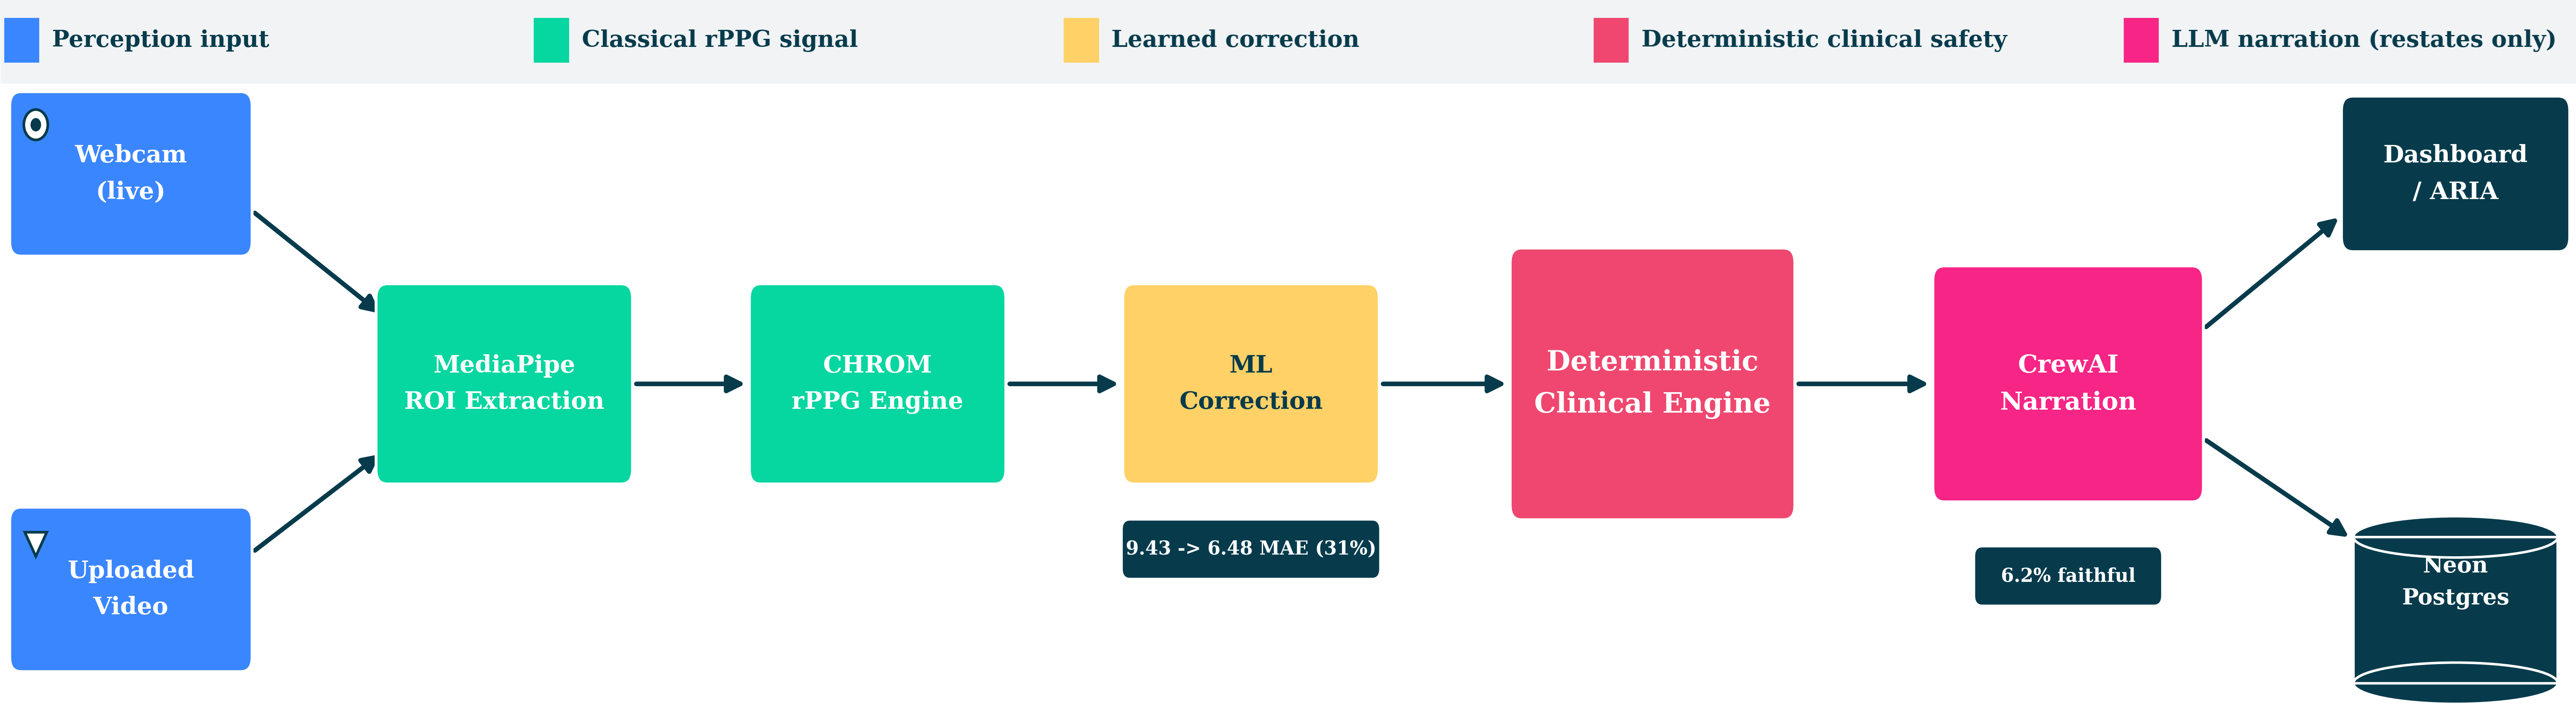
\includegraphics[width=0.97\textwidth]{figures/architecture.png}
{
\footnotesize
\caption{VITAL's end-to-end pipeline. Blue: Perception input (webcam or uploaded video). Teal: The rPPG signal chain. Amber: the learned correction layer. Coral: the deterministic clinical engine -- the sole source of truth for ESI-style acuity, the Compensated Shock flag, and priority score. Pink: the CrewAI narration layer, which only restates and explains that output and never computes or overrides it. Badges mark the two numbers that motivate this separation: a 31\% MAE reduction from the correction layer, and 6.2\% narration faithfulness for the one field a prior revision let the LLM compute unsupervised (Sec.~\ref{sec:faithfulness}).}
}
\label{fig:architecture}
\end{figure*}

\subsection{\textbf{Overview}}
VITAL is organized as \textbf{three layers} against a live Flask API and Next.js dashboard, backed by Neon Postgres. A \textbf{perception layer} extracts a face ROI via MediaPipe Face Mesh (Haar-cascade fallback) and feeds normalized RGB means into an rPPG DSP engine. A \textbf{clinical-reasoning layer} computes ESI-style acuity, a Compensated Shock flag, and a priority score deterministically. A \textbf{narration layer} -- a three-agent CrewAI pipeline -- restates that output for the dashboard and for ARIA, a voice-enabled assistant with read-only database access. Fig.~\ref{fig:architecture} summarizes the pipeline.

\subsection{\textbf{Perception Layer}}
MediaPipe's \cite{b_mediapipe} \textbf{468-point Face Mesh} isolates forehead and malar-cheek landmarks with yaw-aware gating so an off-angle cheek region is excluded rather than averaged in noisily. The layer also estimates \textbf{ambient luminance} and \textbf{centroid drift} per frame, exposed to the correction model as candidate features.

\subsection{\textbf{rPPG DSP Engine}}
The default projection is \textbf{CHROM} \cite{b_chrom}: per-channel normalization, projection onto two chrominance axes, and adaptive scaling by the projected-signal standard-deviation ratio. A \textbf{Welch periodogram} locates the dominant heart-rate frequency; \textbf{cubic-spline upsampling to 250 Hz} supports RMSSD-based HRV; a bandpass (0.10-0.50 Hz) extracts respiratory rate. \textbf{POS} \cite{b_pos_principles} is a hot-swappable alternative, \textbf{not wired into any live route} (Section~\ref{sec:pos-results}).

\subsection{\textbf{Deterministic Clinical Engine}}
\label{sec:clinical-engine}
The \textbf{deterministic clinical scoring module} computes \textbf{ESI-style acuity}, the \textbf{Compensated Shock flag}, and a \textbf{1-100 priority score} directly from extracted vitals in plain deterministic code -- \textbf{not sampled from an LLM}. Rather than a boolean gate that simply checks whether heart rate exceeds 100 bpm and respiratory rate exceeds 20 breaths/min, which treats a barely-elevated reading identically to a severe crisis, severity above that gate is graded by a \textbf{multiplicative interaction}:
\begin{align}
\text{tachy}_{HR} &= \text{ramp}(HR,\ \text{threshold}=100,\ \text{span}=40) \\
\text{tachy}_{RR} &= \text{ramp}(RR,\ \text{threshold}=20,\ \text{span}=15) \\
\text{shock}_{\text{interaction}} &= \text{tachy}_{HR} \times \text{tachy}_{RR}
\end{align}
where $\text{ramp}(v, t, s)$ rises linearly from 0 to 1 as $v$ climbs from $t$ to $t+s$. Multiplying rather than averaging or OR-ing means \textbf{risk accumulates only when both vitals are elevated together}, matching the physiological definition of \emph{compensated} shock as a combined cardiorespiratory response. HRV (RMSSD) and a \textbf{Baevsky Stress Index} are folded in as secondary, lower-weight terms, and \textbf{any Compensated Shock flag unconditionally forces mandatory manual review}. We describe this deliberately as a \textbf{custom, vitals-only scoring rule}, not a faithful ESI \cite{b_esi} or NEWS2 \cite{b_news2} implementation: both require inputs (chief complaint, SpO$_2$, blood pressure, temperature) unmeasurable via webcam alone.

\subsection{\textbf{Multi-Agent Narration Layer}}
Three CrewAI agents run in sequence: a \textbf{Perception Agent} restates already-extracted vitals; a \textbf{Diagnostic Agent} explains the ESI level and shock flag, grounded in retrieved guideline context; a \textbf{Coordinator Agent} restates the priority score for the queue. Guideline grounding uses \textbf{local term-frequency cosine similarity}, simpler than comparable RAG pipelines \cite{b_liu_tsai_cds}. Each request builds a \textbf{fresh set of agents, tasks, and a crew}, since CrewAI's task objects store output internally and are not safe to re-enter concurrently.

\textbf{Why the LLM does not compute the ESI level.} An earlier revision let the agents freely generate the ESI level and shock flag as JSON, falling back to a hardcoded default of 3 on any parse failure -- making \textbf{the single most safety-critical number in the system non-deterministic}. Section~\ref{sec:faithfulness} presents the measurement that motivated reverting this. The live camera path holds one global camera/session (one workstation, one webcam) and is single-stream; uploaded-video runs execute concurrently.

\subsection{\textbf{Dashboard Interface}}
Fig.~\ref{fig:dashboard} shows the two primary dashboard views: \textbf{Vitals Monitor} (top), exposing the live intake feed, optical physiology indicators, and rPPG waveform panel; and \textbf{Triage Dispatch} (bottom), the central queue sorted by acuity. Both are shown idle (hardware disconnected, queue empty), captured before a live acquisition run.

\begin{figure}[ht]
\centering
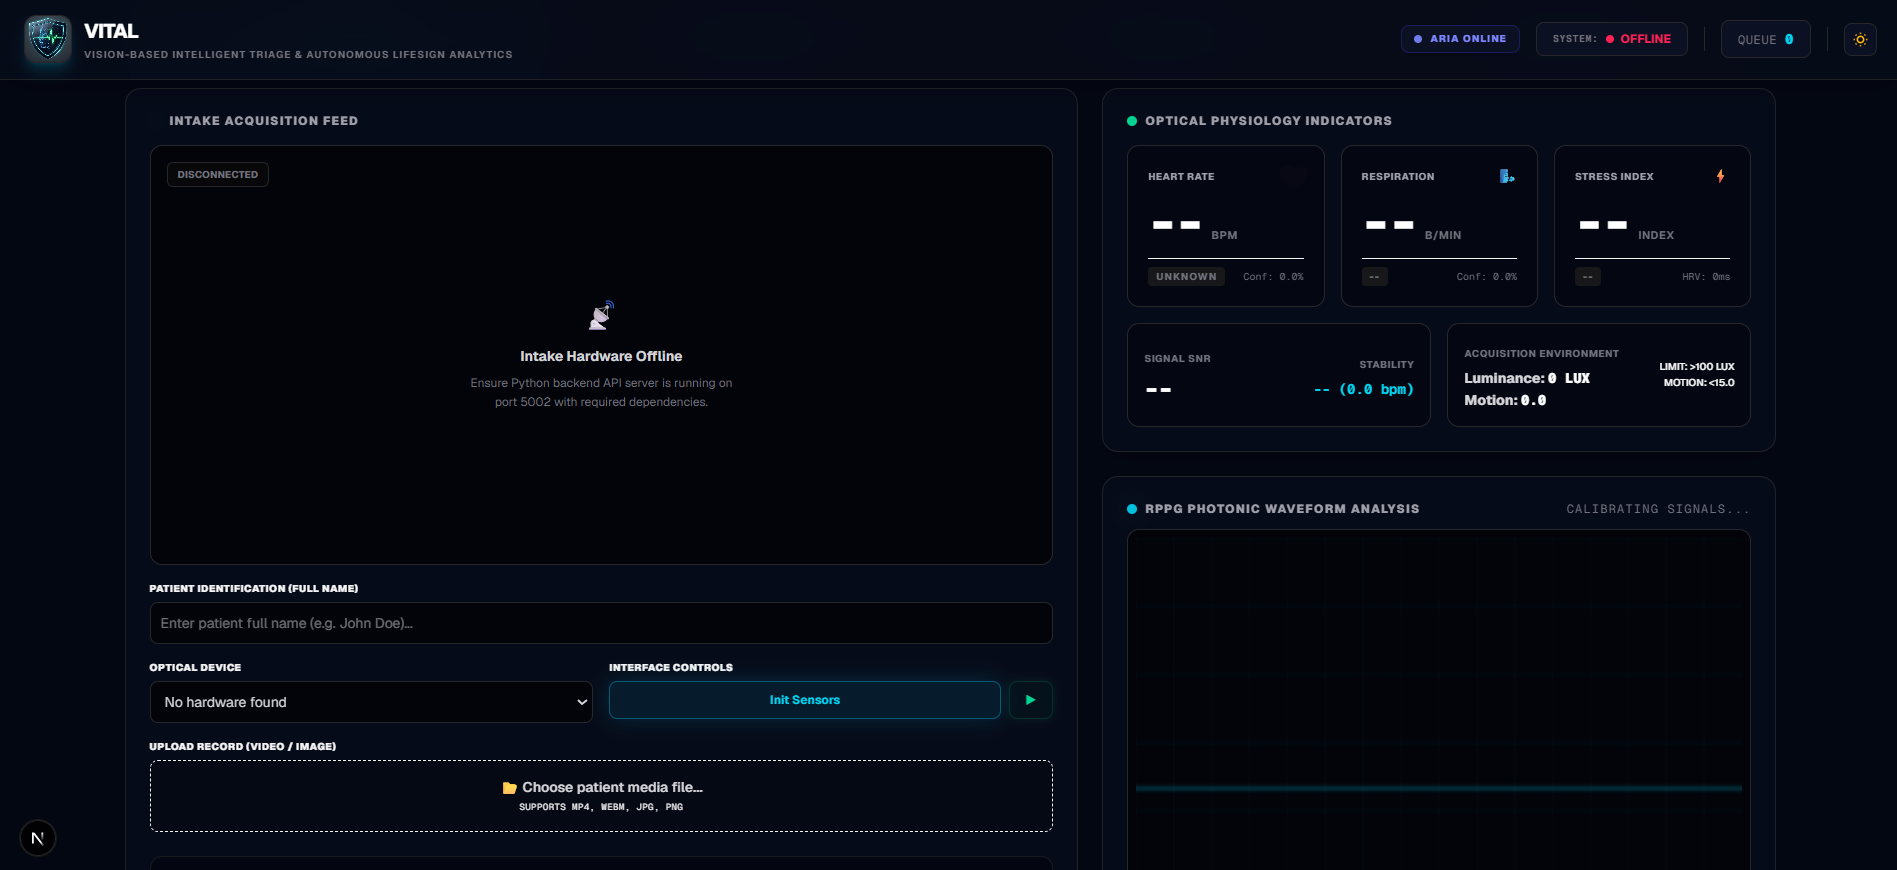
\includegraphics[width=0.85\linewidth]{figures/dashboard_vitals_monitor.png}\\[0.5em]
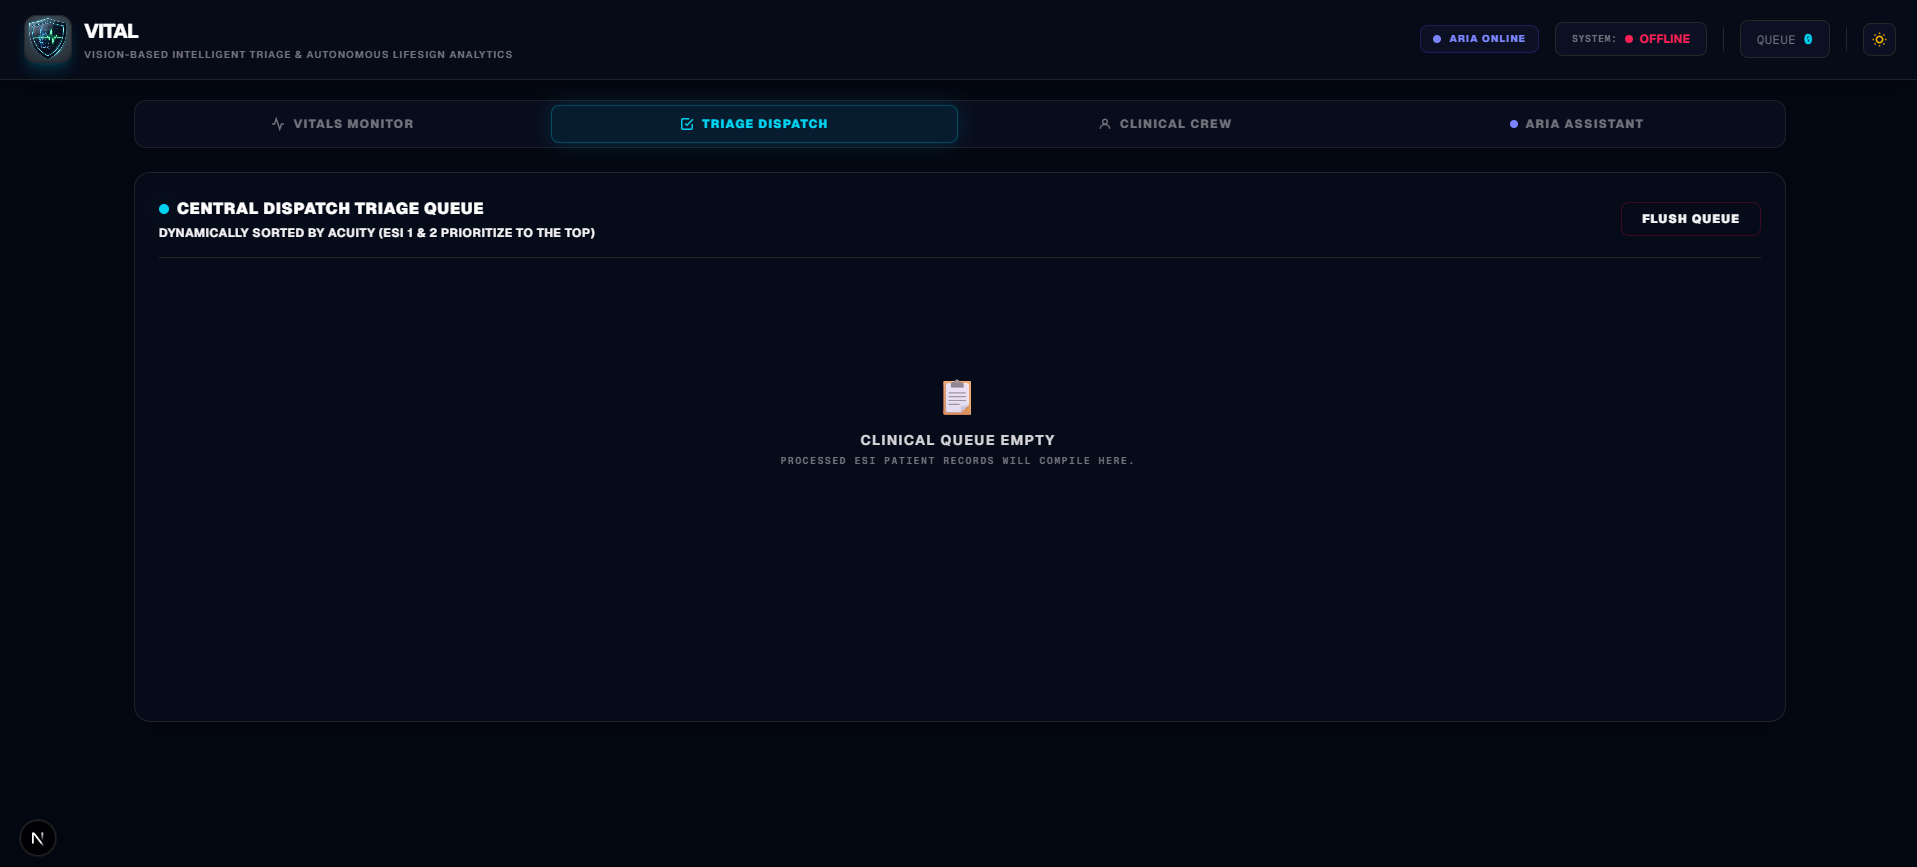
\includegraphics[width=0.85\linewidth]{figures/dashboard_triage_dispatch.png}
\caption{VITAL's dashboard interface. Top: the Vitals Monitor view, showing the intake feed, optical physiology indicators, and rPPG waveform panel. Bottom: the Triage Dispatch view, showing the acuity-sorted central queue. Both panels are captured in their idle state (no active acquisition session), not populated with live measurement data.}
\label{fig:dashboard}
\end{figure}

\section{\textbf{Dataset Description}}

Real-video validation uses \textbf{71 sessions across 51 unique subjects}, pooled from two public datasets \cite{b_ubfc_rppg, b_ubfc_phys}:
\begin{itemize}
    \item \textbf{UBFC-rPPG} \cite{b_ubfc_rppg} -- \textbf{41 sessions} (both public releases combined), a math-stress protocol with ground truth from a contact pulse-oximeter waveform (\texttt{gtdump.xmp}/\texttt{ground\_truth.txt}).
    \item \textbf{UBFC-Phys} \cite{b_ubfc_phys} -- \textbf{30 sessions} (10 subjects $\times$ 3 conditions: rest, speech, arithmetic, following a Trier Social Stress Test-inspired protocol), ground truth from a wrist-worn blood volume pulse (BVP) waveform, peak-detected into a per-session BPM.
\end{itemize}
Class composition across conditions is uneven by design (10 rest, 10 speech, 10 arithmetic, 41 unlabeled UBFC-rPPG), reported stratified rather than pooled into a misleading average (Table~\ref{tab:per-condition}). All model validation uses \textbf{GroupKFold by subject identifier}: no subject's sessions appear in both folds, preventing the correction model from \textbf{memorizing a specific person} rather than learning a general correction.

\section{\textbf{Methodology}}
\label{sec:methodology}

\subsection{\textbf{Classical DSP Bug-Fixing, By Tracing Individual Failures}}
Rather than tuning global thresholds against an aggregate metric, each bug below was found by tracing one specific failing real subject to a root cause, then verified against the full real-video set. Table~\ref{tab:bugs} summarizes the three found bugs.

\begin{table}[h]
\centering
\caption{Classical DSP Bugs, Root-Caused and Fixed}
\label{tab:bugs}
\begin{tabular}{@{}p{1.7cm}p{2.7cm}p{3.5cm}@{}}
\toprule
\textbf{Bug} & \textbf{Root Cause} & \textbf{Fix, Verified Effect (BPM)} \\
\midrule
Harmonic lock-on & Peak-picker locks onto half the true rate for sustained stretches & Promote to the double when it has comparable power; subj.41 52.6$\to$8.2, subj.46 41.2$\to$1.3, subj.9 60.9$\to$2.8 \\
Hardcoded frame rate & Every engine assumed 30 fps regardless of the real source rate & Read the true source fps; subj.25 23.5$\to$3.5, subj.26 25.5$\to$2.5 \\
History freeze & An 18 BPM noise-rejection gate can anchor on an early wrong burst forever & Allow re-anchoring only while the anchor is still small; subj.37 21.0$\to$6.0, no regression elsewhere \\
\bottomrule
\end{tabular}
\end{table}

The history-freeze fix earned a second look: a first attempt fixed its target subject but \textbf{silently regressed the harmonic-lock-on fix's flagship case} back to a 41.8 BPM error, revealing the earlier ``fixed'' result had actually been propped up by this same freeze bug anchoring correctly by luck, not design. The corrected, narrower fix resolved both without re-breaking either. Combined, all three fixes moved the original 56-session real-video baseline from \textbf{17.4 to 8.4 BPM MAE (52\% relative reduction)}; RMSE 24.1$\to$15.6.

\begin{figure}[ht]
\centering
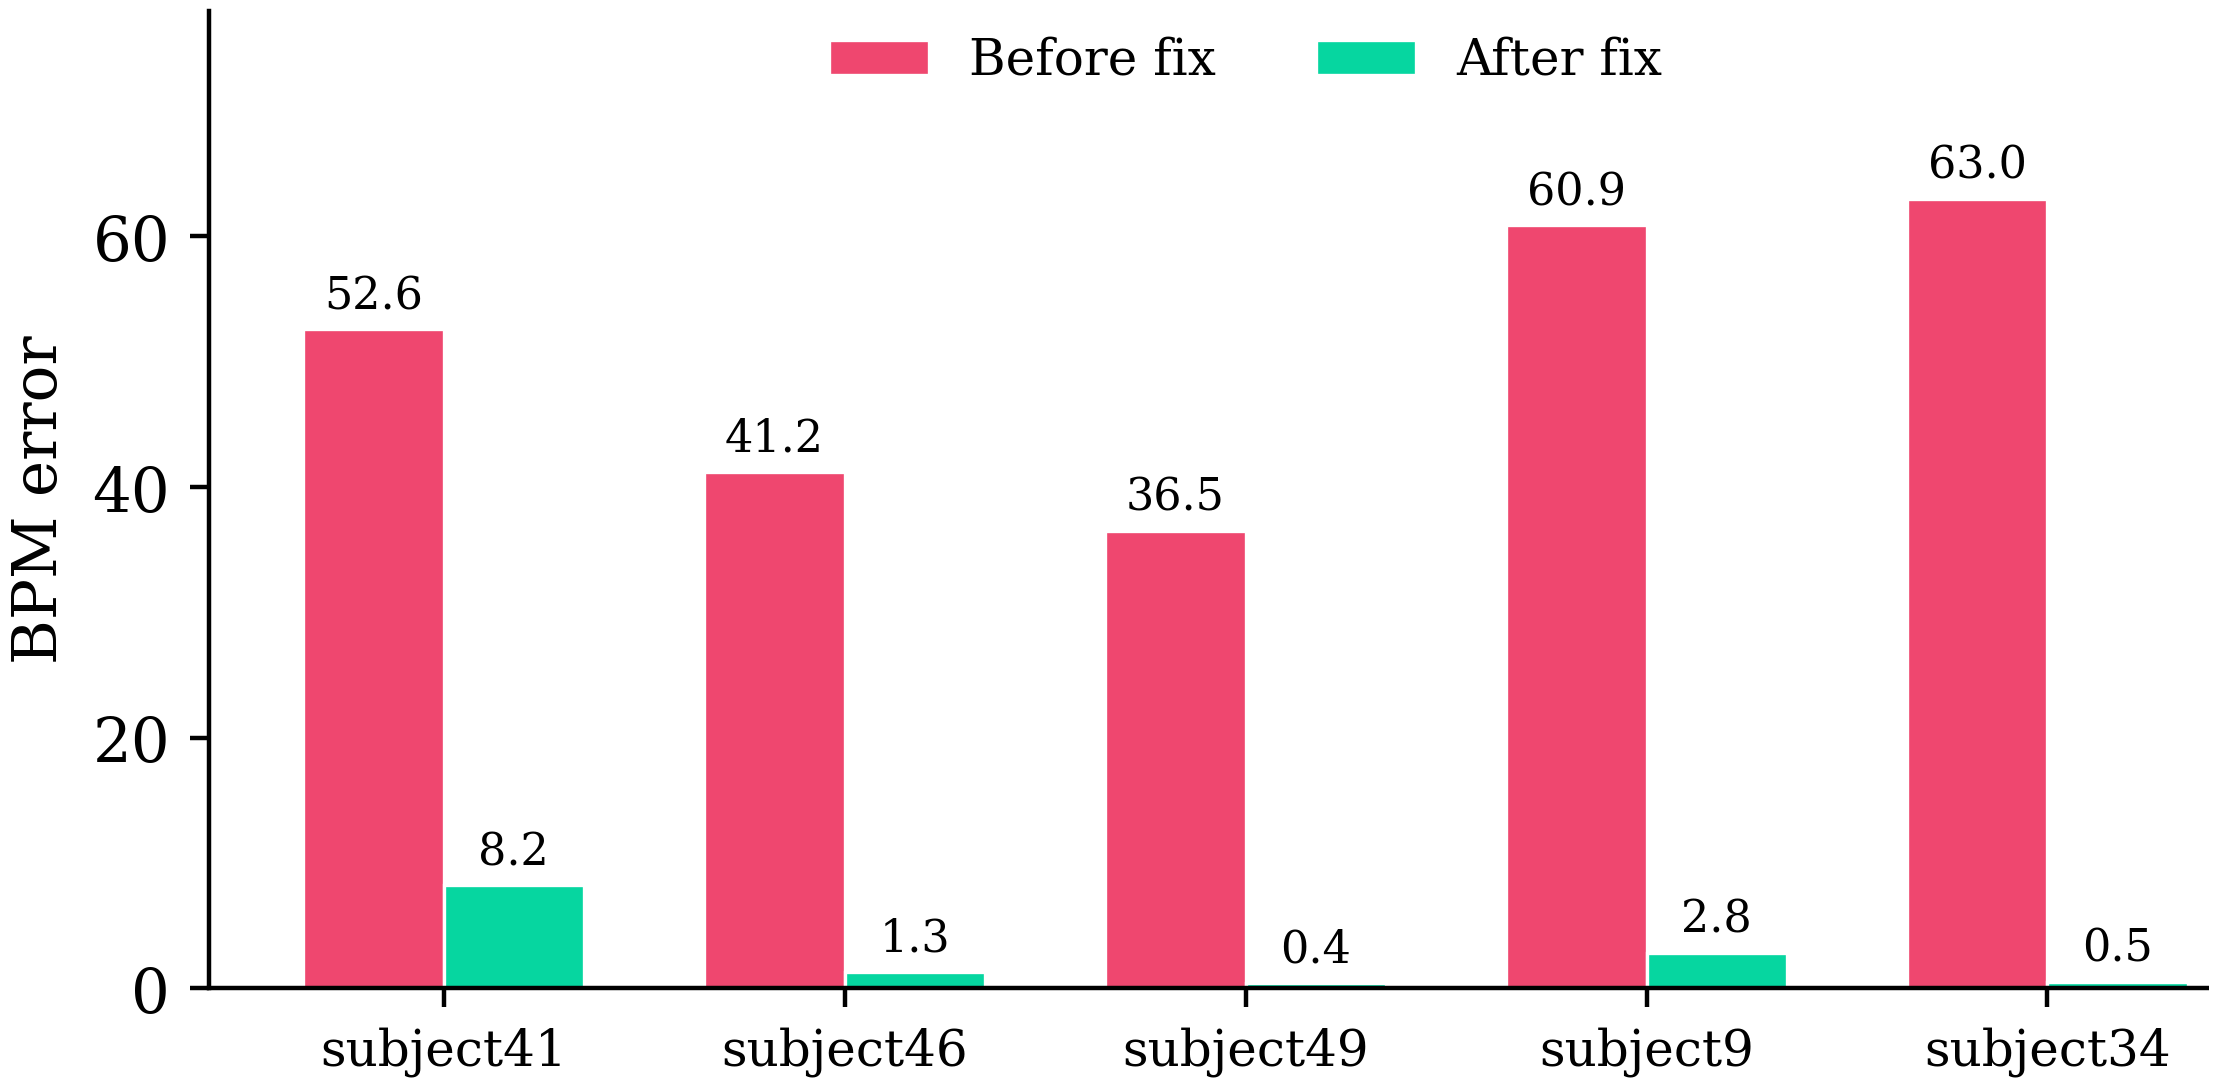
\includegraphics[width=\linewidth]{figures/harmonic_fix_subjects.png}
\caption{Per-subject BPM error before and after the subharmonic-promotion fix for the harmonic lock-on bug. Zero effect on the shipped CHROM synthetic MAE (0.29, unchanged).}
\label{fig:harmonic-fix}
\end{figure}
Fig.~\ref{fig:harmonic-fix} shows this fix's effect on the five subjects it was verified against.

\subsection{\textbf{Hybrid Classical-DSP + ML Correction}}
A \textbf{gradient-boosted regressor} (\texttt{GradientBoostingRegressor}, \textbf{Huber loss}) is trained to correct the classical CHROM pipeline's per-cycle BPM output, using \textbf{ten features per cycle}: raw BPM, signal-quality index, SNR (dB), a stability score, respiratory rate and its confidence, HRV, the Baevsky stress index, and the adaptive filter's low/high cutoff frequencies. The model is evaluated with \textbf{5-fold GroupKFold by subject}, and every session-level result reported in Section~\ref{sec:results} uses a model that \textbf{never saw that subject during training}. Huber loss was adopted after comparing it against squared-error loss on the same folds; it produced a small but consistent improvement (\textbf{8.80$\to$8.67 BPM} per-cycle MAE, \textbf{6.65$\to$6.48 BPM} session-level MAE), consistent with squared-error over-weighting a handful of extreme-outlier sessions. Larger models -- a bigger regularized neural network, a bigger gradient-boosted model, and an ensemble of both -- \textbf{did not outperform the small deployed model}; the binding constraint is \textbf{51 unique subjects}, not the number of labeled cycles.

\subsection{\textbf{POS's Own Bug, Partially Fixed}}
\label{sec:pos-results}
POS \cite{b_pos_principles} exhibits a \textbf{mirror-image failure to CHROM's}: it overshoots to roughly double the true rate from cold start, rather than undershooting. A symmetric ``demote to the half'' check, added to the same peak-selection logic as CHROM's fix, cut POS's synthetic MAE from \textbf{26.71 to 16.00 BPM (28.88 RMSE)} with zero effect on CHROM's own numbers -- a \textbf{real, partial fix}: two of seven synthetic cases still fail. On real video (tested for the first time here), results were mixed: one subject was accurate (1.7 BPM error), but two others failed in opposite directions, and \textbf{threshold tuning could not fix either} -- one subject's true rate never appears as a spectral candidate at all, and the other's correct candidate is present but weak (median \textbf{11\% power}, never crossing an aggressive 30\% threshold). This traces to a \textbf{structural gap}: CHROM applies global mean-normalization and per-buffer variance equalization before projecting; POS applies only per-window mean-normalization, consistent with its literature description as lacking CHROM's stronger illumination compensation \cite{b_qaadan}. Closing this needs a rewrite of POS's projection math, not its peak-selection heuristics; it remains \textbf{experimental and out of the live product}.

\subsection{\textbf{Agent Narration Faithfulness Evaluation}}
\label{sec:faithfulness}
To test whether the LLM narration layer can be trusted with clinical numbers directly, we ran the real CrewAI pipeline (live API calls to an \textbf{8-billion-parameter} instruction-tuned LLM, not a mock) against \textbf{8 controlled clinical scenarios} spanning the acuity range -- normal, isolated tachycardia, isolated tachypnea, mild shock, severe shock, bradycardia, low signal-quality, and no-signal -- each run twice (\textbf{16 total runs}), checking whether the LLM's final JSON output \textbf{exactly matched the deterministic assessment on every field}, despite the task instructions explicitly stating to restate the given values verbatim and not recompute them.

\section{\textbf{Experimental Results}}
\label{sec:results}

\subsection{\textbf{Synthetic Self-Test}}
Table~\ref{tab:synthetic} isolates the DSP math from camera capture and face detection, using a physiologically-modeled synthetic RGB trace across seven known-BPM trials (50-140 BPM, 2\% sensor noise).

\begin{table}[h]
\centering
\caption{Synthetic Validation (DSP Core Only)}
\label{tab:synthetic}
\begin{tabular}{@{}lcc@{}}
\toprule
\textbf{Algorithm} & \textbf{MAE (BPM)} & \textbf{RMSE (BPM)} \\
\midrule
CHROM (shipped default) & \textbf{0.29} & 0.53 \\
POS (experimental, not wired in) & 16.00 & 28.88 \\
\bottomrule
\end{tabular}
\end{table}

\subsection{\textbf{Real-Video Classical vs. Hybrid Accuracy}}
Table~\ref{tab:main-results} reports the headline result across all 71 real sessions; the correction model is always tested on subjects it has never seen before, so it can't simply have memorized their patterns.

\begin{table}[h]
\centering
\caption{Real-Video Accuracy, 71 Sessions / 51 Subjects}
\label{tab:main-results}
\begin{tabular}{@{}lcc@{}}
\toprule
\textbf{Pipeline} & \textbf{MAE (BPM)} & \textbf{RMSE (BPM)} \\
\midrule
Classical DSP only (CHROM) & 9.43 & 16.51 \\
\textbf{Hybrid (DSP + ML correction)} & \textbf{6.48} & \textbf{9.66} \\
\midrule
Relative MAE reduction & \multicolumn{2}{c}{31\%} \\
\bottomrule
\end{tabular}
\end{table}

\begin{table}[h]
\centering
\caption{Per-Condition Accuracy Breakdown}
\label{tab:per-condition}
\begin{tabular}{@{}lccc@{}}
\toprule
\textbf{Condition} & \textbf{Classical} & \textbf{Hybrid} & \textbf{n} \\
\midrule
Speech (talking) & 21.0 & \textbf{7.8} & 10 \\
Arithmetic (mental stress) & 10.4 & \textbf{7.0} & 10 \\
UBFC-rPPG (unlabeled task) & 7.4 & 6.1 & 41 \\
Rest & 5.1 & 6.1 (worse) & 10 \\
\bottomrule
\end{tabular}
\end{table}

\begin{figure}[ht]
\centering
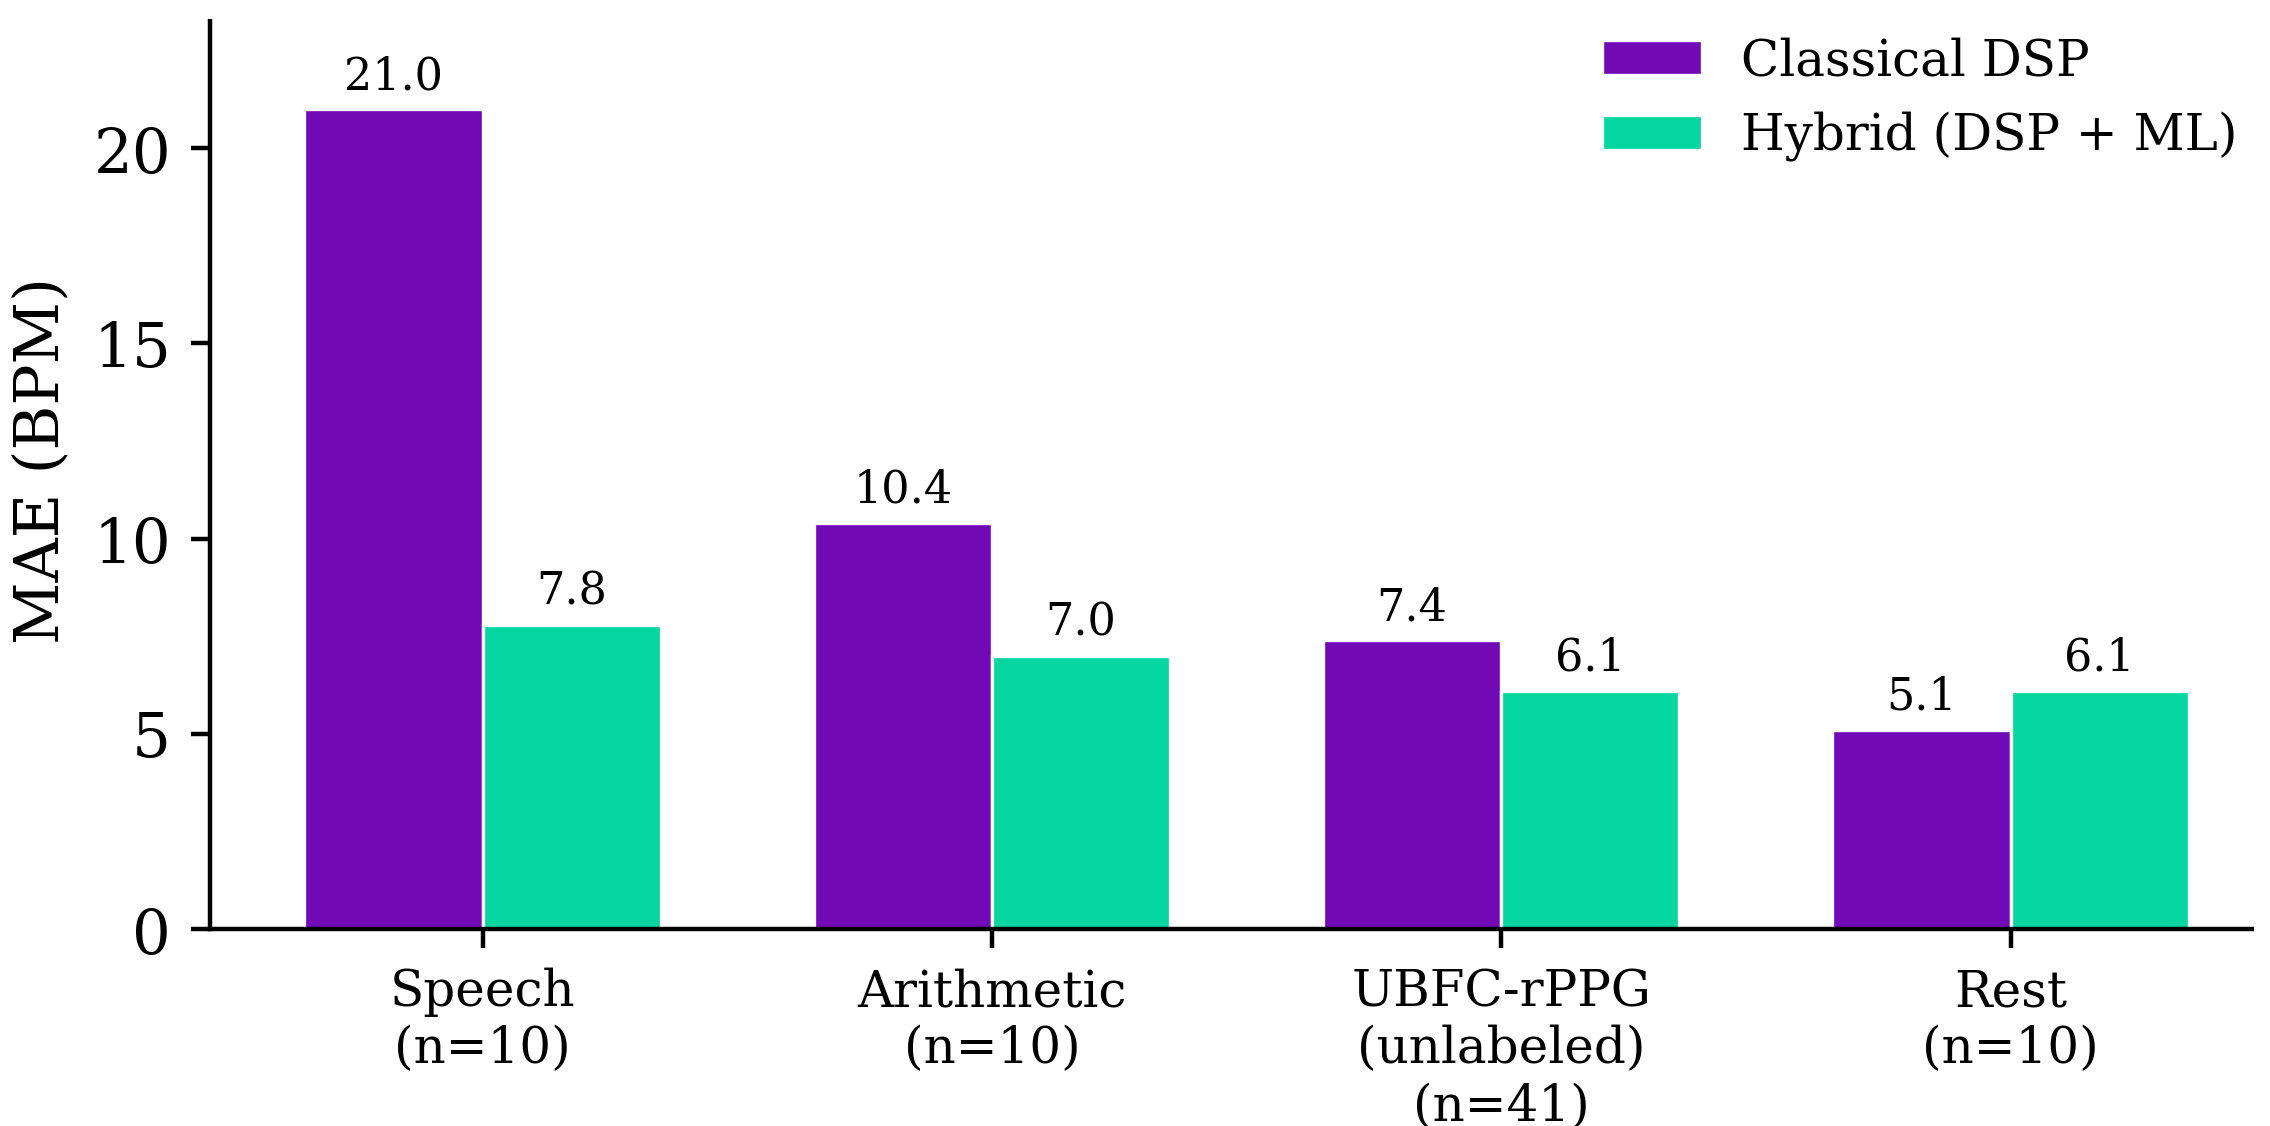
\includegraphics[width=\linewidth]{figures/per_condition_mae.png}
\caption{Classical vs. hybrid MAE by condition. The hybrid model's gain is concentrated in speech and arithmetic; on already-clean rest it is slightly worse, since there is little systematic bias left for it to correct.}
\label{fig:per-condition}
\end{figure}

The hybrid model helps every condition except already-clean rest, where the classical baseline has little bias left to correct (Fig.~\ref{fig:per-condition}). \textbf{Its largest single gain is in speech} -- the one condition three independent DSP-level bug fixes never touched, since mouth-movement motion artifact is a fundamentally different failure mode from frequency-domain harmonic ambiguity or a frame-rate mismatch.

\subsection{\textbf{Comparison Against the Closest Published Benchmark}}
Table~\ref{tab:qaadan-compare} restricts the comparison to the UBFC-rPPG-only subset directly comparable to Qaadan et al.'s evaluation \cite{b_qaadan}, since their study does not include UBFC-Phys.

\begin{table}[h]
\centering
\caption{Comparison on the UBFC-rPPG-Only Subset}
\label{tab:qaadan-compare}
\begin{tabular}{@{}lc@{}}
\toprule
\textbf{Method} & \textbf{MAE (BPM)} \\
\midrule
This work -- classical DSP only & 7.42 \\
This work -- hybrid (DSP + ML correction) & 6.12 \\
Qaadan et al. -- CHROM + XGBoost (their best) \cite{b_qaadan} & \textbf{4.60} \\
\bottomrule
\end{tabular}
\end{table}

We report this honestly: on the narrow task of rPPG heart-rate accuracy alone, \textbf{their approach currently beats both of ours}, and not by a rounding margin. Their own permutation-importance analysis repeatedly ranks \textbf{skewness, lag-1 autocorrelation, sample entropy, and spectral centroid} among their top CHROM features; none of these are in this project's ten-feature correction schema, which is a \textbf{concrete, named, and currently unclosed gap}. What this project has, that a pure benchmarking study does not, is the remainder of this section.

\subsection{\textbf{Agent Narration Faithfulness}}
Table~\ref{tab:faithfulness} reports the field-level exact-match rate between the LLM's restated output and the deterministic ground truth it was given, across all 16 runs.

\begin{table}[h]
\centering
\caption{LLM Agent Narration Faithfulness (16 runs, 8B-parameter LLM)}
\label{tab:faithfulness}
\begin{tabular}{@{}lc@{}}
\toprule
\textbf{Field} & \textbf{Faithfulness rate} \\
\midrule
JSON parses at all & 15/16 (93.8\%) \\
ESI level restated correctly & 13/16 (81.2\%) \\
\textbf{Priority score restated correctly} & \textbf{1/16 (6.2\%)} \\
Shock flag restated correctly & 15/16 (93.8\%) \\
Diagnosis text -- exact wording & 6/16 (37.5\%) \\
Diagnosis text -- correct meaning, different words & 12/16 (75.0\%) \\
\bottomrule
\end{tabular}
\end{table}

\begin{figure}[ht]
\centering
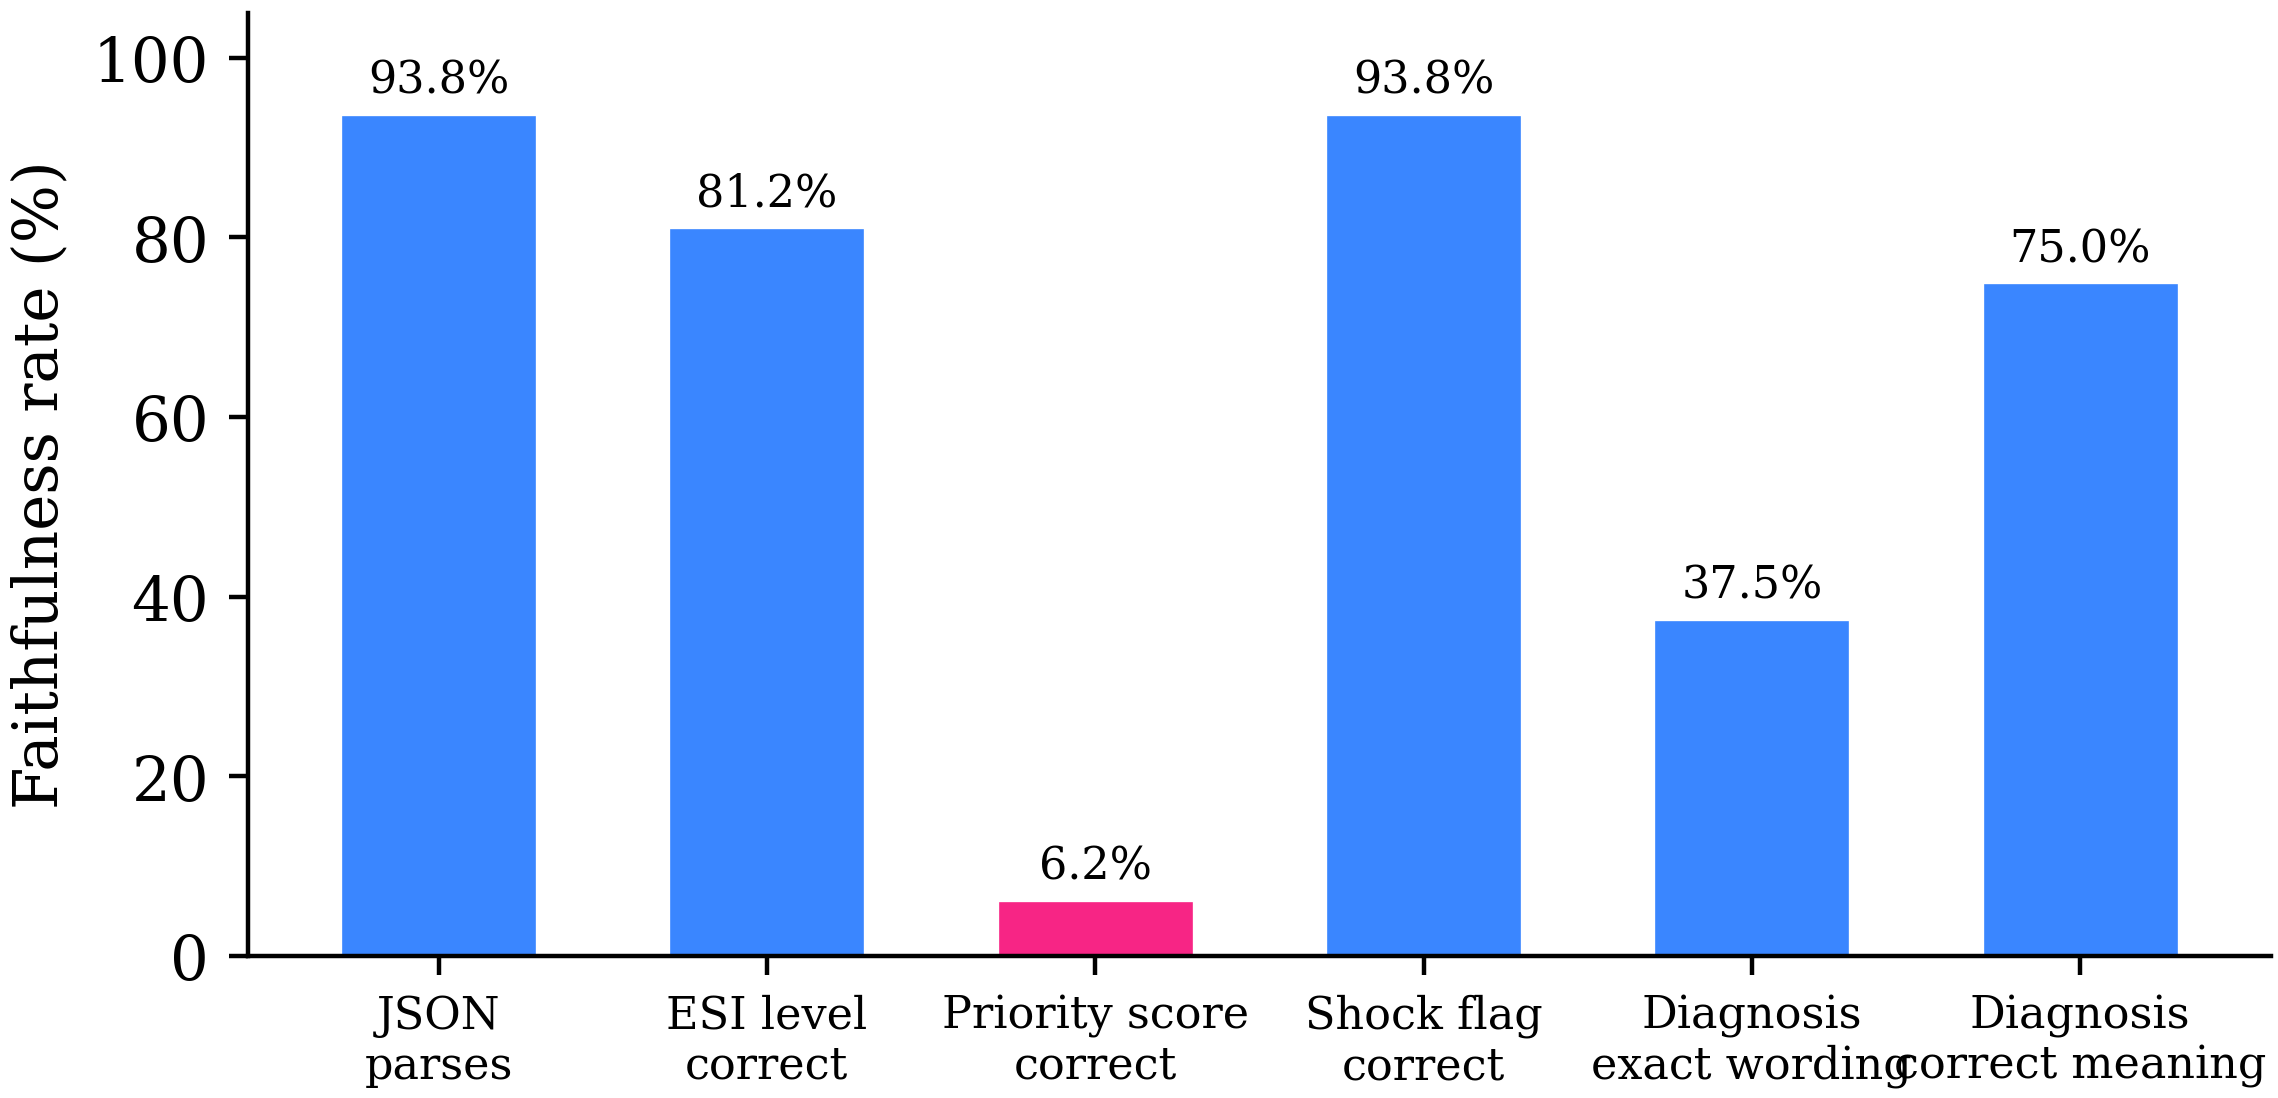
\includegraphics[width=\linewidth]{figures/agent_faithfulness.png}
\caption{LLM agent narration faithfulness by field, 16 runs. The priority score (highlighted) is the one field an earlier system revision let the LLM compute unsupervised; it is also the field the LLM restates least reliably.}
\label{fig:faithfulness}
\end{figure}

Even under an explicit ``restate this exact number, do not recompute it'' instruction, \textbf{the LLM almost never produced a clean, correct integer} for the priority score -- it repeatedly embedded descriptive text in the field instead (e.g. \texttt{"priority\_score": "ESI Level 2 -- Emergent / Compensated Shock (score=0.311)"}). A related finding from the same runs: the LLM occasionally \textbf{attempted to call tools that do not exist} in this system at all, a second, independent reliability gap in the agent layer.

\section{\textbf{Discussion}}

\subsection{\textbf{What the Numbers Actually Mean}}
The result in Table~\ref{tab:faithfulness} is not a defensive-programming assumption -- it is a measurement that this architectural safety rule was \textbf{necessary, not merely cautious}. Had this system trusted the LLM's own JSON output for the priority score, it would have assigned the wrong queue priority to a patient in \textbf{more than 9 of every 10 runs}. Comparable agentic-orchestration architectures build in procedural guardrails against exactly this kind of failure without ever measuring how often an agent's output diverges from ground truth \cite{b_warrier_agentic}; this is what that divergence rate looks like, measured, on a real pipeline.

The hybrid model's largest gain sits exactly where DSP-level fixes could not reach: motion artifact from speech is \textbf{orthogonal} to harmonic ambiguity, frame-rate mismatch, and history-aggregation freeze, so a learned correction absorbs a bias pattern no peak-selection heuristic can express. This also explains why bigger models did not help further: the limiting factor is \textbf{51 subjects}, not the volume of labeled cycles.

\subsection{\textbf{Positioning and Limitations}}
This is deliberately \textbf{not framed as an accuracy paper} competing on a single metric. Qaadan et al.'s study is a pure rPPG-accuracy benchmark with no deployed system, no clinical-safety layer, and no agent-reliability measurement; Table~\ref{tab:qaadan-compare} states plainly that they currently win on their own metric. Real limits remain: \textbf{no real-data respiratory-rate accuracy}, since none of the three datasets provide RR ground truth; \textbf{no skin-tone-stratified accuracy}, since none ship compatible Fitzpatrick metadata; the live-camera path is \textbf{single-session}, so the dashboard's ``queue'' is a sequential log, not concurrent monitoring; and the clinical engine is a \textbf{custom vitals-only rule}, not a validated ESI or NEWS2 implementation \cite{b_esi, b_news2}.

\section{\textbf{Conclusion and Future Work}}

VITAL demonstrates a contactless vitals-to-triage pipeline in which a hybrid correction layer \textbf{closes 31\% of the real-video accuracy gap} left by classical rPPG alone (\textbf{9.43$\to$6.48 BPM MAE} across 71 sessions), and in which a deterministic clinical engine is kept as the \textbf{sole source of truth} for triage-critical numbers -- justified by a measurement that the LLM narration layer restates a given priority score correctly only \textbf{6.2\% of the time}. Three root-caused DSP bugs and one partially-fixed POS bug are reported alongside the fixes that did not work, and a real accuracy gap against the closest published benchmark is reported rather than hidden.

Future work: \textbf{closing the named feature gap} against \cite{b_qaadan} (skewness, autocorrelation, sample entropy, spectral centroid); a \textbf{structural rewrite of POS's projection step}; \textbf{skin-tone-stratified validation} once compatible metadata is available; and a \textbf{live, real-patient pilot}, deliberately out of scope here but planned.

\vspace{-16pt}
\begin{thebibliography}{99}
\scriptsize
\setlength{\itemsep}{0pt}
\setlength{\parskip}{0pt}
\setlength{\parsep}{0pt}
\setlength{\topsep}{0pt}

\bibitem{b_qaadan}
S. Qaadan, R. Al Jayyousi, and O. Alkhalaileh, ``A Unified Benchmarking Framework for Classical Machine Learning Based Heart Rate Estimation from RGB and NIR rPPG,'' \emph{Electronics}, vol. 15, no. 1, p. 218, 2026, doi: 10.3390/electronics15010218.

\bibitem{b_chrom}
G. de Haan and V. Jeanne, ``Robust Pulse Rate From Chrominance-Based rPPG,'' \emph{IEEE Transactions on Biomedical Engineering}, vol. 60, no. 10, pp. 2878--2886, Oct. 2013, doi: 10.1109/TBME.2013.2266196.

\bibitem{b_pos_principles}
W. Wang, A. C. den Brinker, S. Stuijk, and G. de Haan, ``Algorithmic Principles of Remote-PPG,'' \emph{IEEE Transactions on Biomedical Engineering}, vol. 64, no. 7, pp. 1479--1491, Jul. 2017, doi: 10.1109/TBME.2016.2609282.

\bibitem{b_ubfc_rppg}
S. Bobbia, R. Macwan, Y. Benezeth, A. Mansouri, and J. Dubois, ``Unsupervised Skin Tissue Segmentation for Remote Photoplethysmography,'' \emph{Pattern Recognition Letters}, 2017, doi: 10.1016/j.patrec.2017.10.017.

\bibitem{b_ubfc_phys}
R. Meziati Sabour \emph{et al.}, ``UBFC-Phys: A Multimodal Database for Psychophysiological Studies of Social Stress,'' \emph{IEEE Transactions on Affective Computing}, 2021, doi: 10.1109/TAFFC.2021.3056960.

\bibitem{b_mediapipe}
C. Lugaresi \emph{et al.}, ``MediaPipe: A Framework for Building Perception Pipelines,'' \emph{arXiv preprint arXiv:1906.08172}, 2019.

\bibitem{b_esi}
N. Gilboy, T. Tanabe, D. Travers, and A. M. Rosenau, \emph{Emergency Severity Index (ESI): A Triage Tool for Emergency Department Care, Version 4. Implementation Handbook 2012 Edition}, AHRQ Publication No. 12-0014, Agency for Healthcare Research and Quality, Rockville, MD, 2011.

\bibitem{b_news2}
Royal College of Physicians, \emph{National Early Warning Score (NEWS) 2: Standardising the Assessment of Acute-Illness Severity in the NHS. Updated Report of a Working Party}, London: RCP, 2017.

\bibitem{b_pirzada_review}
P. Pirzada, A. Wilde, and D. Harris-Birtill, ``Remote Photoplethysmography for Heart Rate and Blood Oxygenation Measurement: A Review,'' \emph{IEEE Sensors Journal}, vol. 24, no. 15, pp. 23436--23453, Aug. 2024, doi: 10.1109/JSEN.2024.3405414.

\bibitem{b_chin_clinical}
J. W. Chin \emph{et al.}, ``Clinical Validation of rPPG-Enabled Contactless Pulse Rate Monitoring Software in Cardiovascular Disease Patients,'' \emph{Bioengineering}, vol. 13, no. 2, p. 246, Feb. 2026, doi: 10.3390/bioengineering13020246.

\bibitem{b_jonatha_iml}
B. Jonatha and F. F. Lubis, ``Interpretable Machine Learning for Emergency Department Triage: A Systematic Literature Review,'' in \emph{2025 15th International Conference on Information \& Communication Technology and System (ICTS)}, 2025, doi: 10.1109/ICTS67612.2025.11369580.

\bibitem{b_yaddaden}
Y. Yaddaden, Y. Benahmed, M.-D. Rioux, and M. Kallel, ``Machine Learning-Based Pre-Diagnosis Tools in Emergency Departments: Predicting Hospitalization, Mortality and Triage Acuity,'' in \emph{2023 IEEE Third International Conference on Signal, Control and Communication (SCC)}, 2023, doi: 10.1109/SCC59637.2023.10527491.

\bibitem{b_liu_tsai_cds}
Y.-K. Liu and Y.-C. Tsai, ``Explainable AI for Trustworthy Clinical Decision Support: A Case-Based Reasoning System for Nursing Assistants,'' in \emph{2024 IEEE International Conference on Big Data (BigData)}, 2024, pp. 6502--6509, doi: 10.1109/BigData62323.2024.10825008.

\bibitem{b_warrier_agentic}
A. Warrier and Abhilash K. S., ``Autonomous Agentic AI for Clinical Workflow Orchestration: Self-Managing Healthcare Operations,'' in \emph{2025 6th International Conference on IoT Based Control Networks and Intelligent Systems (ICICNIS)}, 2025, pp. 1450--1457, doi: 10.1109/ICICNIS66685.2025.11315712.

\bibitem{b_sharma_triagebot}
D. Sharma \emph{et al.}, ``Triage-Bot: An Assistive Triage Framework,'' in \emph{2024 IEEE International Conference on Digital Health (ICDH)}, 2024, pp. 138--140, doi: 10.1109/ICDH62654.2024.00033.

\end{thebibliography}

\end{document}
